
\chapter{Related Works}
Currently, a majority of farmers and insect researchers manually sample insects regularly. Since many insects and mites can be tiny, the samplers must carry tools like digital cameras and 10x magnifying glasses. This monitoring procedure will include traps, beating counts, fecal pellet collection, and more \cite{pinkston}. Though these procedures are successful, maintaining the sampling schedule is troublesome since the researcher/farmer must use different techniques and traps for various insects. For example, to detect and monitor populations of alfalfa weevils, armyworms, and leafhoppers, the recommended guidelines are to do a sweep-net sample twice a week or more \cite{long_goodell_2017}. Moreover, manual sampling can be prone to errors and biases, resulting in inaccurate insect population estimates. Researchers or farmers may miss small insects or misidentify them, leading to incorrect population counts. Additionally, the accuracy of the estimates can be affected by the sampling frequency, location, and timing, as well as the experience of the sampler. These manual sampling limitations can result in delays and errors in the Integrated Pest Management plan.

The Agricultural industry is known for its innovation as farming has improved throughout history for the sake of efficiency. Original manual labor was replaced with machines that increased harvest yields and decreased time spent on many farming processes, including planting, maintenance, and harvesting. Recent advancements in robotic agricultural technology have resulted in the creation of automated harvesting systems that use Deep Learning, sensor-map fields, etc., to replace some of the many manual aspects of agriculture \cite{magee_2020}. Although this principle of automation and technological advancement is exceptionally efficient, it often needs to account for issues like pest control which may be external to the base processes like seeding, growing, and harvesting of arable land.

\section{Automated Farm Management}
Automated farm management systems have expanded their scope to encompass pest monitoring and control, increasing efficiency and accuracy. For instance, Zhang et al. \cite{zhang_bu_wang_2022} developed a system that uses deep learning to identify and count insects on crops within a greenhouse. The system utilizes cameras to capture images and processes them with a convolutional neural network, providing real-time pest data to farmers. This method has the advantage of offering continuous monitoring but may be limited by factors such as camera resolution and lighting conditions. Similarly, an automated pest detection system for crops using unmanned aerial vehicles (UAVs) equipped with cameras and a machine learning-based classification algorithm was proposed, as shown in Fig \ref{fig:2.1} \cite{10.3389/fagro.2021.640885, app13031851}. This approach enables large-scale monitoring and rapid response to pest infestations but may be affected by environmental factors such as wind and weather.

\begin{figure}[H]
\begin{center}
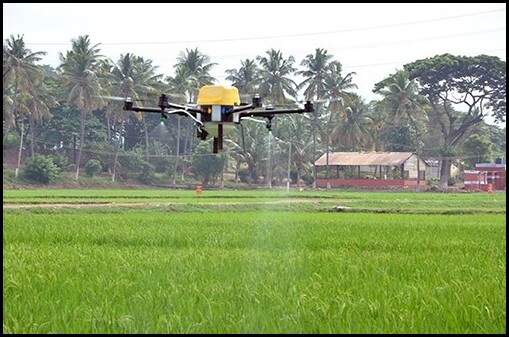
\includegraphics[width=0.85\linewidth]{Honors_Thesis/Figures/2.1.jpg}
\end{center}
\caption{Hexacopter spraying pesticides in Tamil Nadu Agricultural University Farm rice fields in Tamil Nadu, India, during October 2019.}
\label{fig:2.1}
\end{figure}

Additionally, ``Internet of Things" (IoT) based systems have been employed to improve pest management. Qazi et al. \cite{9716089} mention examples of IoT-based smart agriculture systems that integrate pest monitoring with other farm management tasks, such as soil and climate monitoring. By consolidating multiple aspects of farm management, these systems enable an increase in informed decision-making and rapid interventions. However, implementing IoT systems may require significant upfront investment and technical expertise, which may be a barrier for small-scale farmers.

Recent advancements in remote sensing technology have also been employed in pest detection and monitoring. There is an example where remote sensing was used to detect insects in agriculture, focusing on the spectral characteristics of insect sounds \cite{mankin_mccoy_flanders_brandhorst_crocker_shapiro}. This approach can help identify and localize insects in the field but might be limited by the complexity of the acoustic environment and the need for extensive insect sound libraries.

\section{Detection and Classification}
Recent advances in AI and computer vision have facilitated the development of more sophisticated detection and classification methods for insect monitoring. There are examples of efficient deep learning-based approaches being used for detecting and classifying insects through convolutional neural networks (CNNs) \cite{insects14020148}. This method accurately recognizes various insect species, including pests and beneficial insects. However, the performance of such models may be limited by the quality and diversity of the training data, which could lead to misclassifications.

Thenmozhi et al. \cite{THENMOZHI2019104906} developed an automatic recognition system for insect pests using image processing techniques and machine learning classifiers. This approach achieved high recognition rates but required manual preprocessing of images for feature extraction, which could be time-consuming and labor-intensive.

\section{Support Tools}
The emergence of AI-driven support tools has provided farmers and researchers with valuable resources for making educated choices in pest control. Navarro-Hellin et al. \cite{NAVARROHELLIN2016121} created a decision support system that integrates pest monitoring information, meteorological data, and crop growth simulations to deliver customized pesticide application guidance. This system encourages eco-friendly pest management by reducing pesticide use and optimizing crop production.

A pest risk prediction system based on deep learning and remote sensing data was proposed by Chen et al. \cite{CHEN2022107302}. The system predicts the likelihood and severity of pest outbreaks, allowing farmers to implement preventative actions and reduce the consequences of pest infestations. Nevertheless, the precision of these models may be affected by the quality and promptness of input data and the intricacy of the factors that contribute to pest behavior.

Mimicking expert knowledge and decision-making has been an area of interest in research and development across various sectors. Expert systems have been created to help users with tasks that would usually necessitate the skills of a professional, such as medical diagnoses, financial planning, and legal counsel. These systems often employ AI, machine learning, and natural language processing to enable expert-like decision-making and deliver tailored recommendations \cite{durkin1994expert, charniak_mcdermott_1988}.

Expert emulation has been applied to various areas, including pest management in agricultural settings. Gonzalez-Andujar \cite{jose_article}, for example, designed an expert system to estimate the risk of insect pests in olive crops. This system uses specialized knowledge to offer personalized pest management advice based on user-provided information, like plant species and geographic location. Similarly, an expert system for assessing pest risk in organic agriculture was created that assists farmers in recognizing potential hazards and executing suitable pest management tactics \cite{MCKINION198531}.

In addition to conventional expert systems, chatbots have been utilized to replicate expert guidance and offer support in different industries. For instance, Agil-Ifdillah et al. \cite{reset.org_2022} created a chatbot to help farmers identify crop diseases and pests while providing expert suggestions on prevention and treatment methods. This approach enables farmers to access expert knowledge in a more accessible and user-friendly way, lowering the obstacles to adopting sophisticated pest management techniques.
